\begin{figure}[t]
  \centering
  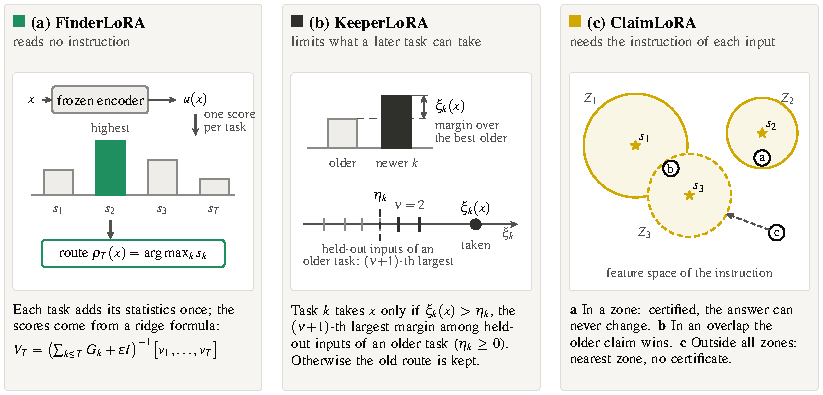
\includegraphics[width=\linewidth]{figures/switch}
  \caption{The three rules that set the route. (a)~\recog{} reads no instruction: it scores every
  task on a frozen feature $u(x)$ of the input with one ridge formula and takes the highest score.
  (b)~\handicap{} adds a handicap for a new task: task $k$ takes an input only if its margin
  $\xi_k(x)$ over the best older task is above $\eta_k$, the $(\nu+1)$-th largest margin among the
  held-out inputs of an older task ($\nu = 2$ in our runs). (c)~\cert{} needs the instruction of
  each input: a task owns a protected zone around the signature of its instruction; an input in a
  zone is certified and belongs to the oldest zone that contains it, and an input outside every
  zone goes to the nearest zone without a certificate.}
  \label{fig:switch}
\end{figure}
